\documentclass[border=12pt]{standalone}
\usepackage{tikz}
\usetikzlibrary{arrows.meta, shapes, calc, positioning, backgrounds, fit}

%% ── Colores ────────────────────────────────────────────────────
\definecolor{grayfill}  {RGB}{241,239,232}
\definecolor{graystroke}{RGB}{ 95, 94, 90}
\definecolor{bluefill}  {RGB}{230,241,251}
\definecolor{bluestroke}{RGB}{ 24, 95,165}
\definecolor{purpfill}  {RGB}{238,237,254}
\definecolor{purpstroke}{RGB}{ 83, 74,183}
\definecolor{tealfill}  {RGB}{225,245,238}
\definecolor{tealstroke}{RGB}{ 15,110, 86}
\definecolor{coralfill} {RGB}{250,236,231}
\definecolor{coralstroke}{RGB}{153, 60, 29}
\definecolor{textsub}   {RGB}{ 90, 88, 84}
\definecolor{divider}   {RGB}{180,178,169}

%% ── Estilos ────────────────────────────────────────────────────
\tikzset{
  blk/.style 2 args={
    rectangle, rounded corners=7pt,
    minimum width=#1, minimum height=1.05cm,
    text width=#1-0.6cm, align=center,
    fill=#2fill, draw=#2stroke, line width=0.4pt,
    font=\sffamily
  },
  blktall/.style 2 args={
    rectangle, rounded corners=7pt,
    minimum width=#1, minimum height=1.55cm,
    text width=#1-0.6cm, align=center,
    fill=#2fill, draw=#2stroke, line width=0.4pt,
    font=\sffamily
  },
  subst/.style={font=\sffamily\footnotesize, text=textsub},
  seclbl/.style={font=\sffamily\tiny\scshape, text=textsub, opacity=0.65,
                 draw=none, fill=none},
  arr/.style={-{Stealth[length=5.5pt,width=4.5pt]}, line width=0.8pt,
              color=textsub},
}

\newcommand{\twolinenode}[4]{
  \node[#2] (#1) {
    \textbf{#3}\\[1pt]
    \textcolor{textsub}{\footnotesize #4}
  };
}

\begin{document}
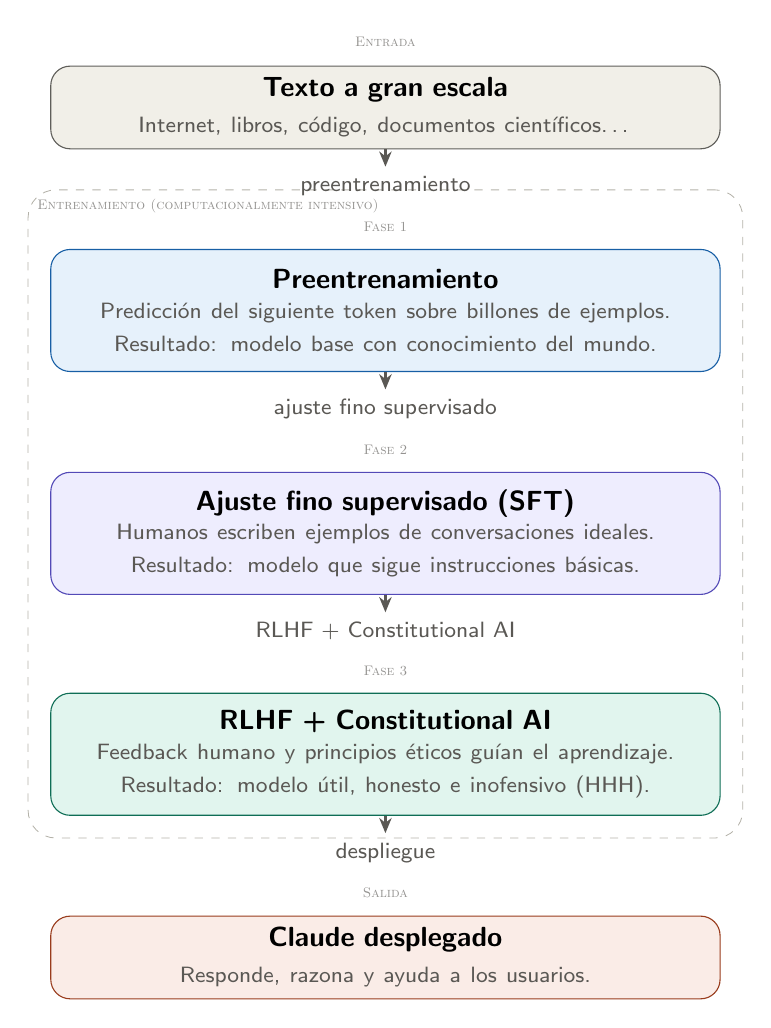
\begin{tikzpicture}[node distance=0.55cm]

%% ── Entrada ────────────────────────────────────────────────────
\node[seclbl] (sec0) {Entrada};

\twolinenode{entrada}{blk={8.5cm}{gray}, below=0.12cm of sec0}
  {Texto a gran escala}
  {Internet, libros, código, documentos científicos…}

\node[subst, below=0.22cm of entrada] (lbl1) {preentrenamiento};
\draw[arr] (entrada.south) -- (lbl1.north);

%% ── Fase 1 ─────────────────────────────────────────────────────
\node[seclbl, below=0.08cm of lbl1] (sec1) {Fase 1};

\twolinenode{fase1}{blktall={8.5cm}{blue}, below=0.1cm of sec1}
  {Preentrenamiento}
  {Predicción del siguiente token sobre billones de ejemplos.\\
   Resultado: modelo base con conocimiento del mundo.}

\node[subst, below=0.22cm of fase1] (lbl2) {ajuste fino supervisado};
\draw[arr] (fase1.south) -- (lbl2.north);

%% ── Fase 2 ─────────────────────────────────────────────────────
\node[seclbl, below=0.08cm of lbl2] (sec2) {Fase 2};

\twolinenode{fase2}{blktall={8.5cm}{purp}, below=0.1cm of sec2}
  {Ajuste fino supervisado (SFT)}
  {Humanos escriben ejemplos de conversaciones ideales.\\
   Resultado: modelo que sigue instrucciones básicas.}

\node[subst, below=0.22cm of fase2] (lbl3) {RLHF + Constitutional AI};
\draw[arr] (fase2.south) -- (lbl3.north);

%% ── Fase 3 ─────────────────────────────────────────────────────
\node[seclbl, below=0.08cm of lbl3] (sec3) {Fase 3};

\twolinenode{fase3}{blktall={8.5cm}{teal}, below=0.1cm of sec3}
  {RLHF + Constitutional AI}
  {Feedback humano y principios éticos guían el aprendizaje.\\
   Resultado: modelo útil, honesto e inofensivo (HHH).}

\node[subst, below=0.22cm of fase3] (lbl4) {despliegue};
\draw[arr] (fase3.south) -- (lbl4.north);

%% ── Salida ─────────────────────────────────────────────────────
\node[seclbl, below=0.08cm of lbl4] (sec4) {Salida};

\twolinenode{salida}{blk={8.5cm}{coral}, below=0.1cm of sec4}
  {Claude desplegado}
  {Responde, razona y ayuda a los usuarios.}

%% ── Cuadro contenedor de las tres fases ───────────────────────
\begin{pgfonlayer}{background}
  \node[draw=divider, line width=0.3pt, rounded corners=10pt,
        fill=none, dashed,
        fit=(sec1)(fase1)(lbl2)(sec2)(fase2)(lbl3)(sec3)(fase3),
        inner sep=8pt] (trainbox) {};
\end{pgfonlayer}
\node[seclbl, anchor=north west] at (trainbox.north west)
  {Entrenamiento (computacionalmente intensivo)};

\end{tikzpicture}
\end{document}
